% Created by tikzDevice version 0.11 on 2018-04-23 15:23:07
% !TEX encoding = UTF-8 Unicode
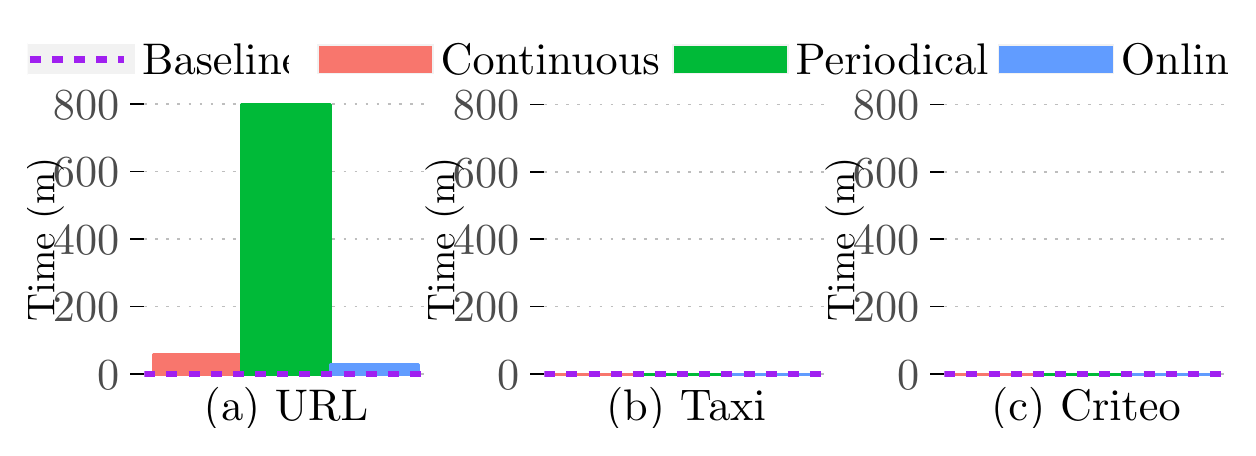
\begin{tikzpicture}[x=1pt,y=1pt]
\definecolor{fillColor}{RGB}{255,255,255}
\path[use as bounding box,fill=fillColor,fill opacity=0.00] (0,0) rectangle (433.62,144.54);
\begin{scope}
\path[clip] (  0.00,  0.00) rectangle (433.62,144.54);
\definecolor{fillColor}{RGB}{255,255,255}

\path[fill=fillColor] (-13.56,121.66) rectangle (108.61,144.54);
\end{scope}
\begin{scope}
\path[clip] (  0.00,  0.00) rectangle (433.62,144.54);
\definecolor{drawColor}{RGB}{255,255,255}
\definecolor{fillColor}{gray}{0.95}

\path[draw=drawColor,line width= 0.6pt,line join=round,line cap=round,fill=fillColor] ( -3.53,127.35) rectangle ( 39.15,138.85);
\end{scope}
\begin{scope}
\path[clip] (  0.00,  0.00) rectangle (433.62,144.54);
\definecolor{drawColor}{RGB}{160,32,240}

\path[draw=drawColor,line width= 2.3pt,dash pattern=on 4pt off 4pt ,line join=round] (  0.74,133.10) -- ( 34.88,133.10);
\end{scope}
\begin{scope}
\path[clip] (  0.00,  0.00) rectangle (433.62,144.54);
\definecolor{drawColor}{RGB}{0,0,0}

\node[text=drawColor,anchor=base west,inner sep=0pt, outer sep=0pt, scale=  1.60] at ( 41.32,127.59) {Baseline};
\end{scope}
\begin{scope}
\path[clip] (  0.00,  0.00) rectangle (433.62,144.54);
\definecolor{fillColor}{RGB}{255,255,255}

\path[fill=fillColor] ( 94.39,121.66) rectangle (447.18,144.54);
\end{scope}
\begin{scope}
\path[clip] (  0.00,  0.00) rectangle (433.62,144.54);
\definecolor{drawColor}{RGB}{0,0,0}

\node[text=drawColor,anchor=base west,inner sep=0pt, outer sep=0pt, scale=  0.00] at (100.08,133.10) {Deployment};
\end{scope}
\begin{scope}
\path[clip] (  0.00,  0.00) rectangle (433.62,144.54);
\definecolor{drawColor}{RGB}{255,255,255}
\definecolor{fillColor}{gray}{0.95}

\path[draw=drawColor,line width= 0.6pt,line join=round,line cap=round,fill=fillColor] (104.41,127.35) rectangle (147.09,138.85);
\end{scope}
\begin{scope}
\path[clip] (  0.00,  0.00) rectangle (433.62,144.54);
\definecolor{drawColor}{RGB}{248,118,109}
\definecolor{fillColor}{RGB}{248,118,109}

\path[draw=drawColor,line width= 1.1pt,line cap=round,fill=fillColor] (105.84,128.78) rectangle (145.67,137.43);
\end{scope}
\begin{scope}
\path[clip] (  0.00,  0.00) rectangle (433.62,144.54);
\definecolor{drawColor}{RGB}{255,255,255}
\definecolor{fillColor}{gray}{0.95}

\path[draw=drawColor,line width= 0.6pt,line join=round,line cap=round,fill=fillColor] (232.68,127.35) rectangle (275.36,138.85);
\end{scope}
\begin{scope}
\path[clip] (  0.00,  0.00) rectangle (433.62,144.54);
\definecolor{drawColor}{RGB}{0,186,56}
\definecolor{fillColor}{RGB}{0,186,56}

\path[draw=drawColor,line width= 1.1pt,line cap=round,fill=fillColor] (234.10,128.78) rectangle (273.93,137.43);
\end{scope}
\begin{scope}
\path[clip] (  0.00,  0.00) rectangle (433.62,144.54);
\definecolor{drawColor}{RGB}{255,255,255}
\definecolor{fillColor}{gray}{0.95}

\path[draw=drawColor,line width= 0.6pt,line join=round,line cap=round,fill=fillColor] (350.21,127.35) rectangle (392.89,138.85);
\end{scope}
\begin{scope}
\path[clip] (  0.00,  0.00) rectangle (433.62,144.54);
\definecolor{drawColor}{RGB}{97,156,255}
\definecolor{fillColor}{RGB}{97,156,255}

\path[draw=drawColor,line width= 1.1pt,line cap=round,fill=fillColor] (351.64,128.78) rectangle (391.47,137.43);
\end{scope}
\begin{scope}
\path[clip] (  0.00,  0.00) rectangle (433.62,144.54);
\definecolor{drawColor}{RGB}{0,0,0}

\node[text=drawColor,anchor=base west,inner sep=0pt, outer sep=0pt, scale=  1.60] at (149.26,127.59) {Continuous};
\end{scope}
\begin{scope}
\path[clip] (  0.00,  0.00) rectangle (433.62,144.54);
\definecolor{drawColor}{RGB}{0,0,0}

\node[text=drawColor,anchor=base west,inner sep=0pt, outer sep=0pt, scale=  1.60] at (277.53,127.59) {Periodical};
\end{scope}
\begin{scope}
\path[clip] (  0.00,  0.00) rectangle (433.62,144.54);
\definecolor{drawColor}{RGB}{0,0,0}

\node[text=drawColor,anchor=base west,inner sep=0pt, outer sep=0pt, scale=  1.60] at (395.06,127.59) {Online};
\end{scope}
\begin{scope}
\path[clip] (  0.00,  0.00) rectangle (144.54,121.66);
\definecolor{drawColor}{RGB}{255,255,255}
\definecolor{fillColor}{RGB}{255,255,255}

\path[draw=drawColor,line width= 0.6pt,line join=round,line cap=round,fill=fillColor] (  0.00, -0.00) rectangle (144.54,121.66);
\end{scope}
\begin{scope}
\path[clip] ( 42.13, 14.51) rectangle (144.54,121.66);
\definecolor{fillColor}{RGB}{255,255,255}

\path[fill=fillColor] ( 42.13, 14.51) rectangle (144.54,121.66);
\definecolor{drawColor}{RGB}{255,255,255}

\path[draw=drawColor,line width= 0.3pt,line join=round] ( 42.13, 31.59) --
	(144.54, 31.59);

\path[draw=drawColor,line width= 0.3pt,line join=round] ( 42.13, 55.99) --
	(144.54, 55.99);

\path[draw=drawColor,line width= 0.3pt,line join=round] ( 42.13, 80.40) --
	(144.54, 80.40);

\path[draw=drawColor,line width= 0.3pt,line join=round] ( 42.13,104.80) --
	(144.54,104.80);
\definecolor{drawColor}{RGB}{190,190,190}

\path[draw=drawColor,line width= 0.6pt,dash pattern=on 1pt off 3pt ,line join=round] ( 42.13, 19.38) --
	(144.54, 19.38);

\path[draw=drawColor,line width= 0.6pt,dash pattern=on 1pt off 3pt ,line join=round] ( 42.13, 43.79) --
	(144.54, 43.79);

\path[draw=drawColor,line width= 0.6pt,dash pattern=on 1pt off 3pt ,line join=round] ( 42.13, 68.19) --
	(144.54, 68.19);

\path[draw=drawColor,line width= 0.6pt,dash pattern=on 1pt off 3pt ,line join=round] ( 42.13, 92.60) --
	(144.54, 92.60);

\path[draw=drawColor,line width= 0.6pt,dash pattern=on 1pt off 3pt ,line join=round] ( 42.13,117.01) --
	(144.54,117.01);
\definecolor{drawColor}{RGB}{255,255,255}

\path[draw=drawColor,line width= 0.6pt,line join=round] ( 61.33, 14.51) --
	( 61.33,121.66);

\path[draw=drawColor,line width= 0.6pt,line join=round] ( 93.33, 14.51) --
	( 93.33,121.66);

\path[draw=drawColor,line width= 0.6pt,line join=round] (125.34, 14.51) --
	(125.34,121.66);
\definecolor{drawColor}{RGB}{248,118,109}
\definecolor{fillColor}{RGB}{248,118,109}

\path[draw=drawColor,line width= 1.1pt,line join=round,fill=fillColor] ( 45.33, 19.38) rectangle ( 77.33, 26.38);
\definecolor{drawColor}{RGB}{0,186,56}
\definecolor{fillColor}{RGB}{0,186,56}

\path[draw=drawColor,line width= 1.1pt,line join=round,fill=fillColor] ( 77.33, 19.38) rectangle (109.34,116.79);
\definecolor{drawColor}{RGB}{97,156,255}
\definecolor{fillColor}{RGB}{97,156,255}

\path[draw=drawColor,line width= 1.1pt,line join=round,fill=fillColor] (109.34, 19.38) rectangle (141.34, 22.93);
\definecolor{drawColor}{RGB}{160,32,240}

\path[draw=drawColor,line width= 2.3pt,dash pattern=on 4pt off 4pt ,line join=round] ( 42.13, 19.38) -- (144.54, 19.38);
\end{scope}
\begin{scope}
\path[clip] (  0.00,  0.00) rectangle (433.62,144.54);
\definecolor{drawColor}{gray}{0.30}

\node[text=drawColor,anchor=base east,inner sep=0pt, outer sep=0pt, scale=  1.60] at ( 33.13, 13.87) {0};

\node[text=drawColor,anchor=base east,inner sep=0pt, outer sep=0pt, scale=  1.60] at ( 33.13, 38.28) {200};

\node[text=drawColor,anchor=base east,inner sep=0pt, outer sep=0pt, scale=  1.60] at ( 33.13, 62.68) {400};

\node[text=drawColor,anchor=base east,inner sep=0pt, outer sep=0pt, scale=  1.60] at ( 33.13, 87.09) {600};

\node[text=drawColor,anchor=base east,inner sep=0pt, outer sep=0pt, scale=  1.60] at ( 33.13,111.50) {800};
\end{scope}
\begin{scope}
\path[clip] (  0.00,  0.00) rectangle (433.62,144.54);
\definecolor{drawColor}{RGB}{0,0,0}

\path[draw=drawColor,line width= 0.6pt,line join=round] ( 37.13, 19.38) --
	( 42.13, 19.38);

\path[draw=drawColor,line width= 0.6pt,line join=round] ( 37.13, 43.79) --
	( 42.13, 43.79);

\path[draw=drawColor,line width= 0.6pt,line join=round] ( 37.13, 68.19) --
	( 42.13, 68.19);

\path[draw=drawColor,line width= 0.6pt,line join=round] ( 37.13, 92.60) --
	( 42.13, 92.60);

\path[draw=drawColor,line width= 0.6pt,line join=round] ( 37.13,117.01) --
	( 42.13,117.01);
\end{scope}
\begin{scope}
\path[clip] (  0.00,  0.00) rectangle (433.62,144.54);
\definecolor{drawColor}{RGB}{0,0,0}

\node[text=drawColor,anchor=base,inner sep=0pt, outer sep=0pt, scale=  1.60] at ( 93.33,  2.49) {(a) URL};
\end{scope}
\begin{scope}
\path[clip] (  0.00,  0.00) rectangle (433.62,144.54);
\definecolor{drawColor}{RGB}{0,0,0}

\node[text=drawColor,rotate= 90.00,anchor=base,inner sep=0pt, outer sep=0pt, scale=  1.40] at (  9.64, 68.09) {Time (m)};
\end{scope}
\begin{scope}
\path[clip] (144.54,  0.00) rectangle (289.08,121.66);
\definecolor{drawColor}{RGB}{255,255,255}
\definecolor{fillColor}{RGB}{255,255,255}

\path[draw=drawColor,line width= 0.6pt,line join=round,line cap=round,fill=fillColor] (144.54, -0.00) rectangle (289.08,121.66);
\end{scope}
\begin{scope}
\path[clip] (186.67, 14.51) rectangle (289.08,121.66);
\definecolor{fillColor}{RGB}{255,255,255}

\path[fill=fillColor] (186.67, 14.51) rectangle (289.08,121.66);
\definecolor{drawColor}{RGB}{255,255,255}

\path[draw=drawColor,line width= 0.3pt,line join=round] (186.67, 31.56) --
	(289.08, 31.56);

\path[draw=drawColor,line width= 0.3pt,line join=round] (186.67, 55.91) --
	(289.08, 55.91);

\path[draw=drawColor,line width= 0.3pt,line join=round] (186.67, 80.26) --
	(289.08, 80.26);

\path[draw=drawColor,line width= 0.3pt,line join=round] (186.67,104.62) --
	(289.08,104.62);
\definecolor{drawColor}{RGB}{190,190,190}

\path[draw=drawColor,line width= 0.6pt,dash pattern=on 1pt off 3pt ,line join=round] (186.67, 19.38) --
	(289.08, 19.38);

\path[draw=drawColor,line width= 0.6pt,dash pattern=on 1pt off 3pt ,line join=round] (186.67, 43.74) --
	(289.08, 43.74);

\path[draw=drawColor,line width= 0.6pt,dash pattern=on 1pt off 3pt ,line join=round] (186.67, 68.09) --
	(289.08, 68.09);

\path[draw=drawColor,line width= 0.6pt,dash pattern=on 1pt off 3pt ,line join=round] (186.67, 92.44) --
	(289.08, 92.44);

\path[draw=drawColor,line width= 0.6pt,dash pattern=on 1pt off 3pt ,line join=round] (186.67,116.79) --
	(289.08,116.79);
\definecolor{drawColor}{RGB}{255,255,255}

\path[draw=drawColor,line width= 0.6pt,line join=round] (205.87, 14.51) --
	(205.87,121.66);

\path[draw=drawColor,line width= 0.6pt,line join=round] (237.87, 14.51) --
	(237.87,121.66);

\path[draw=drawColor,line width= 0.6pt,line join=round] (269.88, 14.51) --
	(269.88,121.66);
\definecolor{drawColor}{RGB}{248,118,109}
\definecolor{fillColor}{RGB}{248,118,109}

\path[draw=drawColor,line width= 1.1pt,line join=round,fill=fillColor] (189.87, 19.38) rectangle (221.87, 19.38);
\definecolor{drawColor}{RGB}{0,186,56}
\definecolor{fillColor}{RGB}{0,186,56}

\path[draw=drawColor,line width= 1.1pt,line join=round,fill=fillColor] (221.87, 19.38) rectangle (253.88, 19.38);
\definecolor{drawColor}{RGB}{97,156,255}
\definecolor{fillColor}{RGB}{97,156,255}

\path[draw=drawColor,line width= 1.1pt,line join=round,fill=fillColor] (253.88, 19.38) rectangle (285.88, 19.38);
\definecolor{drawColor}{RGB}{160,32,240}

\path[draw=drawColor,line width= 2.3pt,dash pattern=on 4pt off 4pt ,line join=round] (186.67, 19.38) -- (289.08, 19.38);
\end{scope}
\begin{scope}
\path[clip] (  0.00,  0.00) rectangle (433.62,144.54);
\definecolor{drawColor}{gray}{0.30}

\node[text=drawColor,anchor=base east,inner sep=0pt, outer sep=0pt, scale=  1.60] at (177.67, 13.87) {0};

\node[text=drawColor,anchor=base east,inner sep=0pt, outer sep=0pt, scale=  1.60] at (177.67, 38.23) {200};

\node[text=drawColor,anchor=base east,inner sep=0pt, outer sep=0pt, scale=  1.60] at (177.67, 62.58) {400};

\node[text=drawColor,anchor=base east,inner sep=0pt, outer sep=0pt, scale=  1.60] at (177.67, 86.93) {600};

\node[text=drawColor,anchor=base east,inner sep=0pt, outer sep=0pt, scale=  1.60] at (177.67,111.28) {800};
\end{scope}
\begin{scope}
\path[clip] (  0.00,  0.00) rectangle (433.62,144.54);
\definecolor{drawColor}{RGB}{0,0,0}

\path[draw=drawColor,line width= 0.6pt,line join=round] (181.67, 19.38) --
	(186.67, 19.38);

\path[draw=drawColor,line width= 0.6pt,line join=round] (181.67, 43.74) --
	(186.67, 43.74);

\path[draw=drawColor,line width= 0.6pt,line join=round] (181.67, 68.09) --
	(186.67, 68.09);

\path[draw=drawColor,line width= 0.6pt,line join=round] (181.67, 92.44) --
	(186.67, 92.44);

\path[draw=drawColor,line width= 0.6pt,line join=round] (181.67,116.79) --
	(186.67,116.79);
\end{scope}
\begin{scope}
\path[clip] (  0.00,  0.00) rectangle (433.62,144.54);
\definecolor{drawColor}{RGB}{0,0,0}

\node[text=drawColor,anchor=base,inner sep=0pt, outer sep=0pt, scale=  1.60] at (237.87,  2.49) {(b) Taxi};
\end{scope}
\begin{scope}
\path[clip] (  0.00,  0.00) rectangle (433.62,144.54);
\definecolor{drawColor}{RGB}{0,0,0}

\node[text=drawColor,rotate= 90.00,anchor=base,inner sep=0pt, outer sep=0pt, scale=  1.40] at (154.18, 68.09) {Time (m)};
\end{scope}
\begin{scope}
\path[clip] (289.08,  0.00) rectangle (433.62,121.66);
\definecolor{drawColor}{RGB}{255,255,255}
\definecolor{fillColor}{RGB}{255,255,255}

\path[draw=drawColor,line width= 0.6pt,line join=round,line cap=round,fill=fillColor] (289.08, -0.00) rectangle (433.62,121.66);
\end{scope}
\begin{scope}
\path[clip] (331.21, 14.51) rectangle (433.62,121.66);
\definecolor{fillColor}{RGB}{255,255,255}

\path[fill=fillColor] (331.21, 14.51) rectangle (433.62,121.66);
\definecolor{drawColor}{RGB}{255,255,255}

\path[draw=drawColor,line width= 0.3pt,line join=round] (331.21, 31.56) --
	(433.62, 31.56);

\path[draw=drawColor,line width= 0.3pt,line join=round] (331.21, 55.91) --
	(433.62, 55.91);

\path[draw=drawColor,line width= 0.3pt,line join=round] (331.21, 80.26) --
	(433.62, 80.26);

\path[draw=drawColor,line width= 0.3pt,line join=round] (331.21,104.62) --
	(433.62,104.62);
\definecolor{drawColor}{RGB}{190,190,190}

\path[draw=drawColor,line width= 0.6pt,dash pattern=on 1pt off 3pt ,line join=round] (331.21, 19.38) --
	(433.62, 19.38);

\path[draw=drawColor,line width= 0.6pt,dash pattern=on 1pt off 3pt ,line join=round] (331.21, 43.74) --
	(433.62, 43.74);

\path[draw=drawColor,line width= 0.6pt,dash pattern=on 1pt off 3pt ,line join=round] (331.21, 68.09) --
	(433.62, 68.09);

\path[draw=drawColor,line width= 0.6pt,dash pattern=on 1pt off 3pt ,line join=round] (331.21, 92.44) --
	(433.62, 92.44);

\path[draw=drawColor,line width= 0.6pt,dash pattern=on 1pt off 3pt ,line join=round] (331.21,116.79) --
	(433.62,116.79);
\definecolor{drawColor}{RGB}{255,255,255}

\path[draw=drawColor,line width= 0.6pt,line join=round] (350.41, 14.51) --
	(350.41,121.66);

\path[draw=drawColor,line width= 0.6pt,line join=round] (382.41, 14.51) --
	(382.41,121.66);

\path[draw=drawColor,line width= 0.6pt,line join=round] (414.42, 14.51) --
	(414.42,121.66);
\definecolor{drawColor}{RGB}{248,118,109}
\definecolor{fillColor}{RGB}{248,118,109}

\path[draw=drawColor,line width= 1.1pt,line join=round,fill=fillColor] (334.41, 19.38) rectangle (366.41, 19.38);
\definecolor{drawColor}{RGB}{0,186,56}
\definecolor{fillColor}{RGB}{0,186,56}

\path[draw=drawColor,line width= 1.1pt,line join=round,fill=fillColor] (366.41, 19.38) rectangle (398.42, 19.38);
\definecolor{drawColor}{RGB}{97,156,255}
\definecolor{fillColor}{RGB}{97,156,255}

\path[draw=drawColor,line width= 1.1pt,line join=round,fill=fillColor] (398.42, 19.38) rectangle (430.42, 19.38);
\definecolor{drawColor}{RGB}{160,32,240}

\path[draw=drawColor,line width= 2.3pt,dash pattern=on 4pt off 4pt ,line join=round] (331.21, 19.38) -- (433.62, 19.38);
\end{scope}
\begin{scope}
\path[clip] (  0.00,  0.00) rectangle (433.62,144.54);
\definecolor{drawColor}{gray}{0.30}

\node[text=drawColor,anchor=base east,inner sep=0pt, outer sep=0pt, scale=  1.60] at (322.21, 13.87) {0};

\node[text=drawColor,anchor=base east,inner sep=0pt, outer sep=0pt, scale=  1.60] at (322.21, 38.23) {200};

\node[text=drawColor,anchor=base east,inner sep=0pt, outer sep=0pt, scale=  1.60] at (322.21, 62.58) {400};

\node[text=drawColor,anchor=base east,inner sep=0pt, outer sep=0pt, scale=  1.60] at (322.21, 86.93) {600};

\node[text=drawColor,anchor=base east,inner sep=0pt, outer sep=0pt, scale=  1.60] at (322.21,111.28) {800};
\end{scope}
\begin{scope}
\path[clip] (  0.00,  0.00) rectangle (433.62,144.54);
\definecolor{drawColor}{RGB}{0,0,0}

\path[draw=drawColor,line width= 0.6pt,line join=round] (326.21, 19.38) --
	(331.21, 19.38);

\path[draw=drawColor,line width= 0.6pt,line join=round] (326.21, 43.74) --
	(331.21, 43.74);

\path[draw=drawColor,line width= 0.6pt,line join=round] (326.21, 68.09) --
	(331.21, 68.09);

\path[draw=drawColor,line width= 0.6pt,line join=round] (326.21, 92.44) --
	(331.21, 92.44);

\path[draw=drawColor,line width= 0.6pt,line join=round] (326.21,116.79) --
	(331.21,116.79);
\end{scope}
\begin{scope}
\path[clip] (  0.00,  0.00) rectangle (433.62,144.54);
\definecolor{drawColor}{RGB}{0,0,0}

\node[text=drawColor,anchor=base,inner sep=0pt, outer sep=0pt, scale=  1.60] at (382.41,  2.49) {(c) Criteo};
\end{scope}
\begin{scope}
\path[clip] (  0.00,  0.00) rectangle (433.62,144.54);
\definecolor{drawColor}{RGB}{0,0,0}

\node[text=drawColor,rotate= 90.00,anchor=base,inner sep=0pt, outer sep=0pt, scale=  1.40] at (298.72, 68.09) {Time (m)};
\end{scope}
\end{tikzpicture}
